% Title:       Multiple documents from one source
% Author:      Leo Arnold
% URL:         https://github.com/leoarnold/eurotex2012-uniflow
% License:     CC BY 4.0 - http://creativecommons.org/licenses/by/4.0/

\documentclass{maps}

\usepackage[english]{babel}
\usepackage[utf8]{inputenc}
\usepackage[T1]{fontenc}

\usepackage{csquotes, hyperref, listings, xcolor}
  \hypersetup{colorlinks = false}
  \lstdefinestyle{arn:lst}{breaklines=true, commentstyle=\itshape\color{gray}, frame=tb, numbers=left, numberstyle=\tiny, stepnumber=1, numbersep=4pt, xleftmargin=10pt, xrightmargin=10pt}
  \lstdefinestyle{arn:lst:bash}{language=Bash, basicstyle=\ttfamily, style=arn:lst}

\renewcommand{\notesname}{Weblinks}

\begin{document}
\title{Multiple documents from one source}
\subtitle{\LaTeX\ for lecturers and teachers}
\author{Leo Arnold}

\maketitle

\begin{abstract}
In general \LaTeX{} will produce only one output document. This paradigm shifts when harnessing the power of the so-called shell escape. We will show how to produce multiple output documents with differing content from one single source document. The principle is developed step by step illustrating a typical application in academic teaching.

Focusing on mathematical problems we then explore two ways of automating calculations by integrating free software into the \LaTeX{} run.
\end{abstract}

\begin{keywords}
mathematics, problem sheet, shell escape
\end{keywords}

\section{The problem with problem sheets}
Composing appealing problem sheets and preparing instructive solutions is a time consuming task. Further time is lost when problems need to be altered after typesetting, requiring updated plots and recalculated solutions. When \LaTeX{} is used, we should optimize our workflow, exploit its capabilities to handle as many tedious tasks as possible.

\subsection{Set up for failure: bad practice}

A typical road to ruin is typesetting problems and solutions in separate files. That way it is hard to keep changes in order or notation in sync. For better comprehension we would also like to have the problem formulation above its solution, but copying them from the problem sheet source will just increase the sync problem.

The exam document class by Philip Hirschhorn \cite{arn:hirschhorn} eliminates the need for two source documents. It defines a \texttt{solution} environment that can be included or hidden via a class option. The solutions are typeset in the source document right after the problem which makes for a very natural workflow and easier debugging. Changes in notation can now be handled globally using the text editors \enquote{replace all} function.

On the other hand, having just one source document requires us to pay close attention: without additional adjustments both versions will compile to the same output file name. In an inattentive moment we might accidentally upload the version with solutions to our website too early, rendering the homework assignments pointless. Also \texttt{exam.cls} may not provide the customization you need, for example if you have to implement a department's corporate design or would like to define a third version of the problem sheet containing additional notes.

\subsection{Getting multiple outputs}

Multiple outputs would usually be achieved by multiple invocations of \LaTeX{}. Before each run we would need to manipulate the source document in order to have differing content. All of this can be done using shell scripts or MakeFiles, but it
\begin{itemize}
\item requires an additional (script or make) file
\item requires non-\TeX{} programs
\item requires knowledge beyond \TeX{}
\item may not be platform independent
\end{itemize}
We will introduce a method that handles these shortcomings using only \texttt{pdflatex}.

\subsection{Requirements for a unified workflow}
As we have already seen, it is crucial to have just one source document to avoid incongruities and have a natural way of typesetting.

Typeset problems will most certainly be reused in future courses. Therefore we would like to be able to copy \& paste parts of the exam with ease. Our approach should also apply to documents that \verb+\input+ problems from another source file.

Finally we want to produce multiple outputs differing in content by a single invocation of \texttt{pdflatex}. Our derivation will assume the following use cases:
\begin{itemize}
\item \textbf{student}\quad problems only
\item \textbf{tutor}\quad problems and their solutions
\item \textbf{corrector}\quad problems, solutions and instructions on grading the students work
\end{itemize}



\section{Designing a unified workflow}

Our goal is to produce multiple output documents with differing content in a single run. Though this might seem impossible at first glance, Ulrike Fischer 
found a way \cite{arn:fischer} to do this using only \texttt{pdflatex}. We will introduce her approach step by step, keeping an eye on platform independence.

Since \texttt{pdflatex Sheet.tex} will only produce \texttt{Sheet.pdf} our task splits into three parts:
\begin{enumerate}
\item Find a way to tell \LaTeX{} which parts of the source file to use and which to ignore
\item Change the file name of the output document in order to be able to produce multiple outputs
\item Produce all versions in just one run of \texttt{pdflatex}
\end{enumerate}

\subsection{Selectively in- \& excluding code}

We would like to wrap code into a \LaTeX{} environment and have
some kind of \enquote{switch} in the document preamble to control
whether to have \LaTeX{} process it or not. This is exactly what \texttt{comment.sty} by Victor Eijkhout \cite{arn:eijkhout} does.

\subsubsection{Usage}

The \texttt{comment} package provides us with two simple commands

\begin{itemize}
\item \verb+\includecomment{foobar}+ \quad
defines the environment \texttt{foobar} whose content will be included
\item \verb+\excludecomment{foobar}+ \quad
defines the environment \texttt{foobar} whose content will be ignored
\end{itemize}

\subsubsection{Example}
A nice feature of environments defined using \texttt{comment.sty}
will not break the line, so we can use them in midsentence.
The minimal example

\begin{lstlisting}[language={[LaTeX]TeX}, style=arn:lst]
\includecomment{truth}
\excludecomment{nonsense}

Knuth started
\begin{truth}
developing \TeX{}
\end{truth}
\begin{nonsense}
using WinWord
\end{nonsense}
in 1977.
\end{lstlisting}

\noindent will just output

\begin{quotation}
\noindent Knuth started developing \TeX{} in 1977.
\end{quotation}

\subsubsection{Implementing our use cases}

Knowing the above, we can easily write a document that matches our use cases, but we would still have to adjust the in- and exclusions before compiling.

To reduce such modifications to a bare minimum we will assign a number to each use case. We can then define a macro \verb+\condition+ that expands to the number and use \verb+\ifcase+ to make the adjustments for corresponding case.

\begin{lstlisting}[language={[LaTeX]TeX}, style=arn:lst, caption={Use case implementation}, label=arn:useifcase]
\RequirePackage{comment}

\includecomment{problem}
\ifcase\condition
  % \condition = 0, student
  \excludecomment{solution}
  \excludecomment{howtograde}
\or % \condition = 1, tutor
  \includecomment{solution}
  \excludecomment{howtograde}
\or % \condition = 2, corrector
  \includecomment{solution}
  \includecomment{howtograde}
\fi
\end{lstlisting}

Now all it takes is defining the value of \verb+\condition+ to control the content of the output.

\subsubsection{Coding discipline}
One could of course implement the above using \verb+\ifnum+ instead. I prefer to use \verb+\ifcase+ here because the cases are \enquote{automatically numbered} in order of appearance. That way I got less confused about which number represents which use case, saving me time on debugging.

\subsection{Rethinking command line calls}

We want to control the version of the output without editing the source document. We could write a wrapper document that defines our \verb+\condition+ macro followed by the actual document code:
\begin{lstlisting}[language={[LaTeX]TeX}, style=arn:lst]
\gdef\condition{0}
\input Sheet.tex
\end{lstlisting}
On second thought we can also pass this code on to \LaTeX{} directly on the command line
\begin{verbatim}
pdflatex "\gdef\condition{0} \input Sheet.tex"
\end{verbatim}
avoiding the additional file.

\subsection{Changing the output file name}
By now we can produce any version of the document by altering a single value but they will still be written to the same output file, thereby overwriting the previous output.

A quick look at \texttt{pdflatex}'s manpage\footnote{\url{http://linux.die.net/man/1/pdflatex}} provides
\begin{verbatim}
pdflatex --jobname="student" Sheet.tex
\end{verbatim}
which will create \texttt{student.pdf} from \texttt{Sheet.tex}.

\subsection{Escaping to the Shell}
We know that \LaTeX{} can write to auxiliary files using output stream.
There is also the special stream 18 which will execute the output on the system shell. 
\begin{verbatim}
\write18{ping tug.org}
\end{verbatim}
This is called \textit{escaping} to the shell. Used like this \LaTeX{} will first read
to the end of the document before writing to the shell. 
If we want the command to be executed immediately when \LaTeX{} reaches that point in the document, we use (see \cite{arn:knuth}, p. 226f)
\begin{verbatim}
\immediate\write18{ping tug.org}
\end{verbatim}
In particular this means we can invoke the commands developed in the previous sections from within one \texttt{pdflatex} run.

\subsubsection{Warning}
Giving \LaTeX{} access to the shell is a gateway for exploits. Hence \verb+\write18+ is disabled by default. You can temporarily enable it using 
\begin{verbatim}
pdflatex --shell-escape Sheet.tex
\end{verbatim}
or permanently by adjusting the configuration\footnote{\url{http://wiki.contextgarden.net/Write18}} of your \TeX{} distribution.

\subsection{The UniFlow principle}
After introducing all the building blocks we are now able to understand Ulrike Fischer's ingenious construction \cite{arn:fischer} to produces multiple output documents in one single run.

We start off with a document skeleton to demonstrate the recursive nature of the approach.

\begin{lstlisting}[language={[LaTeX]TeX}, style=arn:lst, texcl=true, caption={General UniFlow template}, label=arn:unitemplate]
% Beginning of Sheet.tex
\ifx\condition\undefined
  % Pseudo shell script (listing \ref{arn:pseudoscript})
  \expandafter\stop
\fi

% Use case implementation (listing \ref{arn:useifcase})

% Actual document code begins here
\end{lstlisting}
Processing this code will have \texttt{pdflatex} enter the \verb+\ifx+ block as the macro \verb+\condition+ has not been defined yet. After executing a \enquote{pseudo shell script} \LaTeX{} will first expand the token \verb+\fi+ and then \verb+\stop+ reading. Note that this run will not produce any output.

In the pseudo shell script, we will invoke \texttt{pdflatex} again on this very same document. The file's base name is obtained from \verb+\jobname+ 
\begin{verbatim}
pdflatex "\string\input\space\jobname"
\end{verbatim}
and we told the parser to interpret \verb+\input+ as a \verb+\string+, preventing it from expansion (\cite{arn:knuth}, p. 40).

When we add a definition of \verb+\condition+, \LaTeX{} will ignore the \verb+\ifx+ block, apply the use case settings and output the desired version.

Considering all use cases and the change of job name we arrive at
\begin{lstlisting}[language={[LaTeX]TeX}, style=arn:lst, caption={Pseudo shell script in \LaTeX{}}, label=arn:pseudoscript]
\immediate\write18{
  pdflatex
  --jobname=\jobname-student
  "\gdef\string\condition{0}
  \string\input\space\jobname"}
\immediate\write18{
  pdflatex
  --jobname=\jobname-tutor
  "\gdef\string\condition{1}
  \string\input\space\jobname"}
\immediate\write18{
  pdflatex
  --jobname=\jobname-corrector
  "\gdef\string\condition{2}
  \string\input\space\jobname"}
\end{lstlisting}

Combining the UniFlow template (listing \ref{arn:unitemplate}) with the implementation of the use cases and the corresponding pseudo shell script (listings \ref{arn:useifcase} and \ref{arn:pseudoscript}) we have constructed the single source document \texttt{Sheet.tex}. Enabling shell escape and processing it with \texttt{pdflatex} will result in the three output documents \texttt{Sheet-student.pdf}, \texttt{Sheet-tutor.pdf} and \texttt{Sheet-corrector.pdf}, each of them with the desired specific content. Therefore all of our initial requirements are met and we have developed a unified workflow.

\subsubsection{Pitfall}
Neither the wrapping \texttt{pdflatex} run nor script \ref{arn:pseudoscript} will produce an output file named \texttt{Sheet.pdf}. This can cause error messages when using text editors with built-in PDF viewers like \TeX{}maker and its standard \enquote{quick build} feature.

\subsubsection{Exercise}
If you would like to check your understanding of the UniFlow principle,
try to write a template for this scenario:

A school teacher always designs two slightly different versions A and B of an exam.
She would like to produce the four versions A, B, A with solutions and B with solutions
from a single source document.

\newpage

\section{UniFlow in action}

The UniFlow principle can also serve to integrate external programs into the \LaTeX{} run. Due to the author's background the examples are taken from mathematics.

For applications in other subjects see the Python\TeX{} gallery \cite{arn:poore} or Herbert Voß's article on general source code \cite{arn:voss}.

For the sake of simplicity we now focus on having only one output document. Nevertheless we will still have to define the \verb+\condition+ macro (setting it to an arbitrary string value) whenever we want \texttt{pdflatex} to ignore the \verb+\ifx+ block. The generalization to multiple output versions is left to the reader as an exercise.

\subsection{Linear Algebra using Sage}

Sage is a free and open source computer algebra system. It is best used on Linux since the \enquote{Windows version} is actually an Ubuntu virtual machine image containing Sage.

We will give a tiny demonstration of the \LaTeX{} interface called Sage\TeX{} and its implementation using the UniFlow principle. Further information on Sage\TeX{} can be found in Günter Rau's demonstration \cite{arn:rau} or on the Sage homepage\footnote{\url{http://www.sagemath.org}}.

\subsubsection{How to compile}
Sage\TeX{} works similar to Bib\TeX{}: First we run \LaTeX{} to extract the Sage commands. These are then processed externally with Sage and the results are included in the second \LaTeX{} run.

\begin{lstlisting}[style=arn:lst:bash]
# Extract Sage commands
pdflatex Example.tex
# Process Sage commands
sage Example.sagetex.sage
# Include Sage outputs
pdflatex Example.tex
\end{lstlisting}

\subsubsection{Implementing UniFlow} \strut

\begin{lstlisting}[language={[LaTeX]TeX}, style=arn:lst]
\ifx\condition\undefined
  \immediate\write18{
    pdflatex
    "\gdef\string\condition{0}
    \string\input\space\jobname"}
  \immediate\write18{
    sage "\jobname.sagetex.sage"}
  \immediate\write18{
    pdflatex
    "\gdef\string\condition{0}
    \string\input\space\jobname"}
  \expandafter\stop
\fi
\end{lstlisting}

\subsubsection{Exercise} Calculate the eigenvalues of the matrix

\[ A = \left(\begin{array}{rrr}
19 & 30 & -20 \\
26 & 39 & -26 \\
61 & 93 & -62
\end{array}\right) \]

\subsubsection{Solution}

The characteristic polynomial of $A$ is
\[ \chi_A(x) = x^{3} + 4 x^{2} + 3 x = x \cdot (x + 1) \cdot (x + 3) \]
hence its eigenvalues are
\[ \left[0, -1, -3\right] \]
Using \texttt{sagetex.sty} we just needed to type
\begin{lstlisting}[language={[LaTeX]TeX}, style=arn:lst]
% 'sagesilent' returns no output
\begin{sagesilent}
A = matrix(QQ, [[19,30,-20], [26,39,-26], [61,93,-62]])
p = A.charpoly()
\end{sagesilent}

\[ A = \sage{A} \]
The characteristic polynomial of $A$ is
\[ \chi_A(x) = \sage{p} = \sage{factor(p)} \]
hence the eigenvalues of $A$ are
\[ \sage{A.eigenvalues()} \]
\end{lstlisting}

Note how this assures that the matrix $A$ and the solution will always match in the output document.
This is as foolproof as it gets.



\subsection{Statistics using R and Sweave}

Data plotting techniques play an important role in any statistics course: histograms, q-q plots, boxplots etc. are handy tools to analyze measured data.

R is a free statistics software system available for all common operating systems\footnote{\url{http://www.r-project.org}}. It comes with the plugin Sweave which \enquote{weaves} R (the free successor to S statistics) into \LaTeX{} documents.

We will use an easy example from elementary probability. More advanced examples can be found for example in Uwe Ziegenhagen's demonstration \cite{arn:ziegenhagen} or on Friedrich Leisch's Sweave website\footnote{\url{http://www.statistik.lmu.de/~leisch/Sweave}}.

\subsubsection{How to compile}
As the output of Sweave will be written to \texttt{Example.tex} we change the file name of our document to \texttt{Example.Rnw} (Rnw = \textbf{R} \textbf{n}o\textbf{w}eb). Now we can use \LaTeX{} code as usual and insert R code as \enquote{chunks} using the noweb syntax. The document is then compiled as follows.

\begin{lstlisting}[style=arn:lst:bash]
# Have R process Example.Rnw and
# create / overwrite Example.tex
R CMD Sweave Example.Rnw
pdflatex Example.tex
\end{lstlisting}

\subsubsection{Implementing UniFlow}\strut

\begin{lstlisting}[language={[LaTeX]TeX}, style=arn:lst]
% Beginning of Example.Rnw
\ifx\condition\undefined
  \immediate\write18{
    R CMD Sweave \jobname.Rnw}
  \immediate\write18{
    pdflatex
    "\gdef\string\condition{0}
    \string\input\space\jobname"}
  \expandafter\stop
\fi
\end{lstlisting}

Editing the \texttt{Example.Rnw} as source file and using the above code, the correct command line call is
\begin{verbatim}
pdflatex --shell-escape Example.Rnw
\end{verbatim}
If you like to use the tab completion feature of your system shell,
it will probably only offer you the \texttt{.tex} file.
Observe that this will generate the same output because both execute the same pseudo shell script.

\subsubsection{Exercise}
Roll a dice 100 times in a row recording the number of pips each time. Visualize their relative frequency as a histogram and a pie chart.

\subsubsection{Solution}
Since this exercise depends on probability, everyone will have a different result. Mine looks like this:

\begin{tabular}{cc}
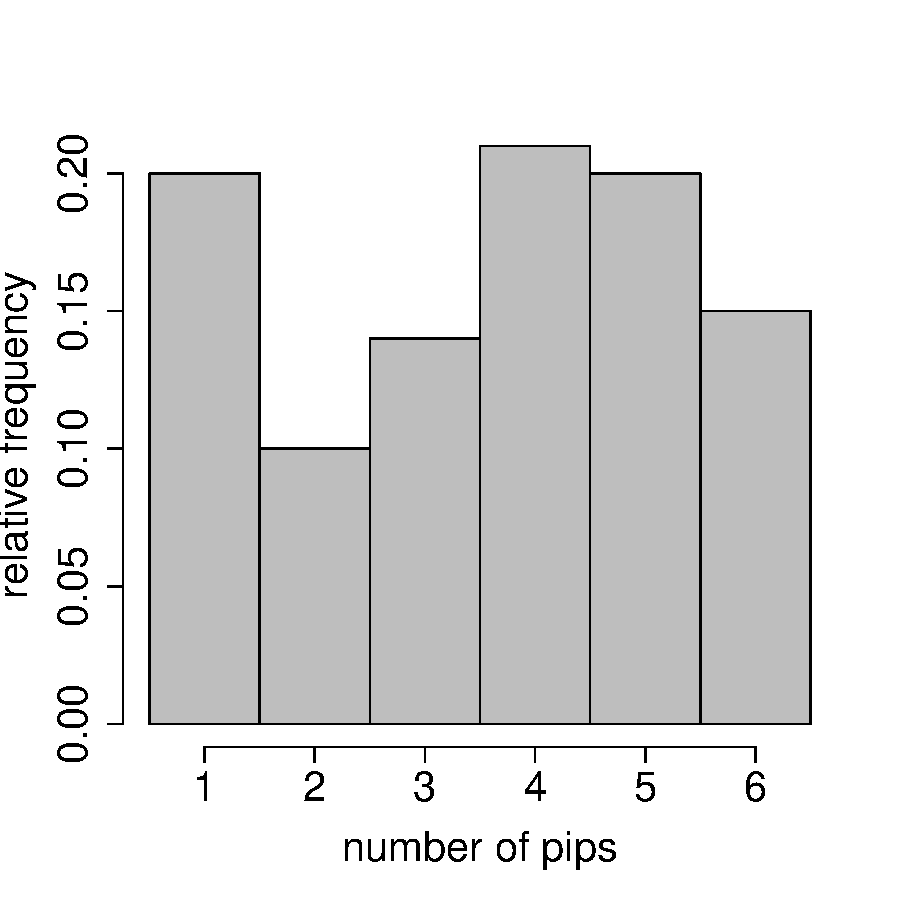
\includegraphics[width=.4\linewidth]{arn/R-hist}
& 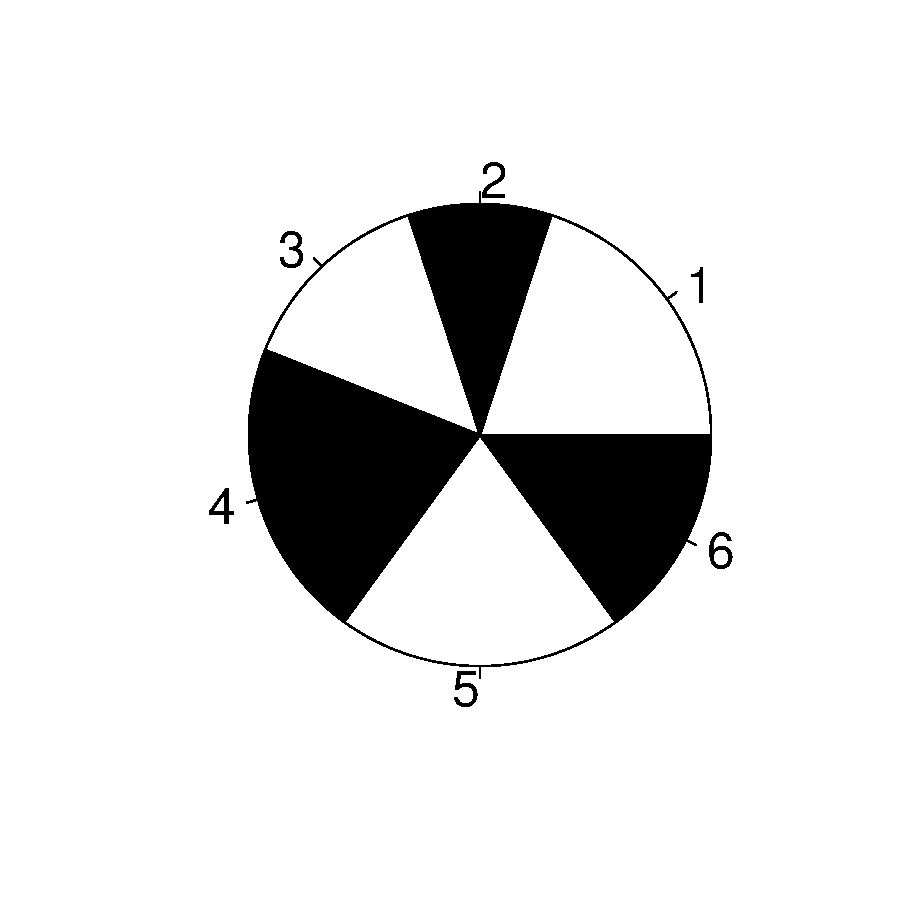
\includegraphics[trim={90 90 60 70},clip=true,width=.4\linewidth]{arn/R-pie}
\end{tabular}

These diagrams where of course generated at compile time from the following code snippet.

\begin{lstlisting}[language=R, style=arn:lst]
# Relevant part of Example.Rnw
<< echo=FALSE, fig=TRUE >>=
par(ps=20)
pips <- sample(1:6,100,replace=TRUE)
hist(pips, breaks=c(0.5, 1.5, 2.5, 3.5, 4.5, 5.5, 6.5), col="gray", freq=FALSE, main="", xlab="number of pips", ylab="relative frequency")
@

<< echo=FALSE, fig=TRUE >>=
pie(table(pips), col=c("white", "black"), cex=2)
@
\end{lstlisting}

Here, due to the use of \textbf{sample}(), the output will be different after every compile run.



\section{Aftermath}

Of course we could have achieved all of this in a one-call fashion using some kind of shell script, \texttt{make}\footnote{\url{http://www.gnu.org/software/make}} or its \LaTeX{} analogs \texttt{latexmk}\footnote{\href{http://ctan.org/tex-archive/support/latexmk/}{\texttt{CTAN:support/latexmk}}} or \texttt{rubber}\footnote{\url{https://launchpad.net/rubber}}.
On the other hand the UniFlow principle provides a platform independent, script-like alternative without additional (Make)files or non-\TeX{} executables.

\subsection{The future of UniFlow}
To enable anyone to implement the UniFlow principle with ease I will work on developing it into a \LaTeX{} package.

Versatility is UniFlow's biggest asset and every reader will by now have his or her special use case in mind -- and most certainly be struggling with the inconvenient syntax of the corresponding \verb+\write18+
statement. Hence designing an intuitive command structure will be key and your \TeX{}nical comments and pieces of advice are always welcome.

One step further we could think about a unified interface to integrate virtually any program into the \LaTeX{} run. Herbert Voß \cite{arn:voss} already showed how general source code can be extracted from a document and reincluding the output after processing. His approach works with any kind of batching method, allowing for an integration into UniFlow (once devolped).

\subsection{Acknowledgments}

Many people have directly or indirectly contributed in the development of the UniFlow principle.

First and foremost I want to thank Ulrike Fischer who provided the core concepts in her short and effective post on StackExchange.

When I was struggling with selectively showing or hiding content, Rolf Niepraschk pointed out the fascinating simplicity of \texttt{comment.sty} to me.

Marcus Bitzl is an avid reader of \enquote{Die \TeX{}nische Komödie} and drew my attention to the articles on the integration of free math software. He was also the first to encourage the development of a UniFlow package.

The articles by Günter Rau (Sage\TeX{}) and Uwe Ziegenhagen (Sweave) were invaluable primers to me and made the vivid demonstrations of UniFlow in action possible.

Finally I would like to express my gratitude to the Euro\TeX{} 2012 organizers for arranging a wonderful and inspiring conference and giving me the opportunity to present the UniFlow principle.

\theendnotes

\bibliographystyle{abbrv}
\bibliography{arn/ET2012-Proc-Arnold}

\end{document}